\newpage
\section{Experiments}

\subsection{Input reading by chunks}\label{input-reading}

\begin{itemize}
  \item \href{https://medium.com/@anuragv.1020/chunk-by-chunk-tackling-big-data-with-efficient-file-reading-in-chunks-c6f7cf153ccd}{Chunk-by-Chunk: Tackling Big Data with Efficient File Reading in Chunks}
  \item \href{https://pkg.go.dev/github.com/apache/arrow/go/arrow/csv#NewReader}{csv chunk reader - with Apache Arrow package}
\end{itemize}

\subsubsection{Apache Arrow}

\href{https://pkg.go.dev/github.com/apache/arrow/go/v12@v12.0.1/arrow/csv}{Apache arrow CSV}
package allows reading csv in chunks of $n$ rows, called \emph{records}.

The thing is that \emph{records} / apache arrow is optimized storing the data in a columnar way (by columns). So that we can not access the original $n$ rows easily, but instead the columns of these rows. And therefore, from them we will need to reconstruct the rows by taking the corresponding elements from each of the columns, given the index of the corresponding row.

Good references:
\begin{itemize}
  \item \href{https://www.apachecon.com/acna2022/slides/01_Topol_Arrow_and_Go.pdf}{Apache Arrow and Go - Good tutorial}
\end{itemize}


\subsubsection{encoding/csv}

\subsubsection{Experiments over the different approaches}

Approaches:
\begin{itemize}
  \item \texttt{1-apache/arrow} direct reading of corresponding data type in the worker.
  \item \texttt{2apache/arrow} reading as string data type. Later conversion in main.
  \item \texttt{3-encoding/csv}: row by row reading and passing chunks of rows to main.
\end{itemize}

\textcolor{red}{TODO: put a schema of the main/worker to show the different approaches better}

\begin{itemize}
  \item For the different approaches we tried with different sizes of files: $10^4$, $10^5$ and $10^6$ number of rows (transactions).
  \item For each of the sizes we compared the time it took to read the full file to each of the variants, testing for different chunk sizes in terms of the number of rows: ranging from $10^0, 10^1, 10^2,...$ up to the total number of rows of the file (maximum possible chunk size, all at once).
  \item Each of the experiments is done 20 times to obtain stable measurements.
  \item \textcolor{red}{WITH HOW MANY CORES?, RAM? -- They were done in the logincluster node!, not with sbatch controlling the number of cores! - check the characteristics of the logincluster!}
\end{itemize}


\begin{figure}[H]
  \centering
  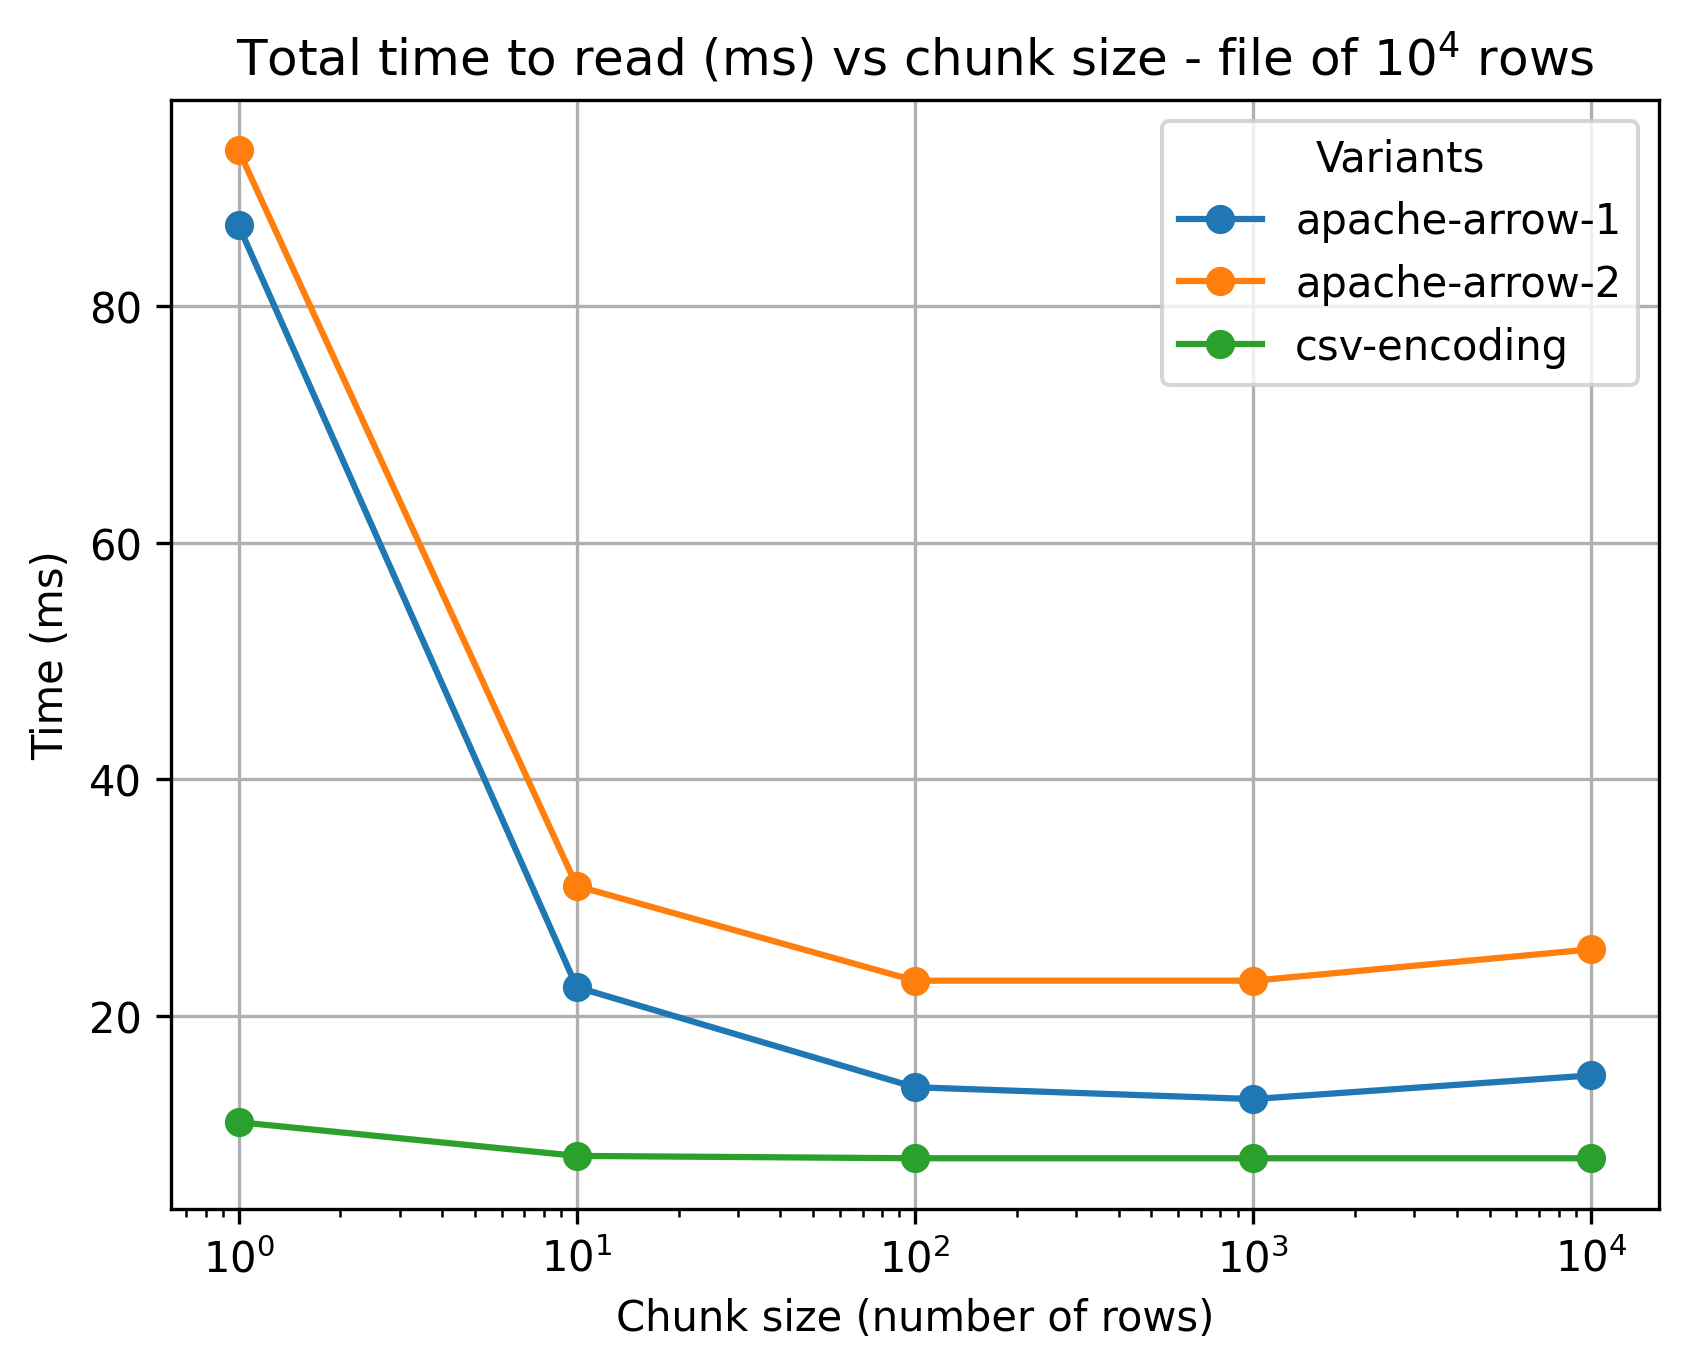
\includegraphics[scale = 0.7]{images/4-Experiments/read-input-10-4.png}
  \caption{Comparison of the variants for file of $10^4$ rows}
\end{figure}

\begin{figure}[H]
  \centering
  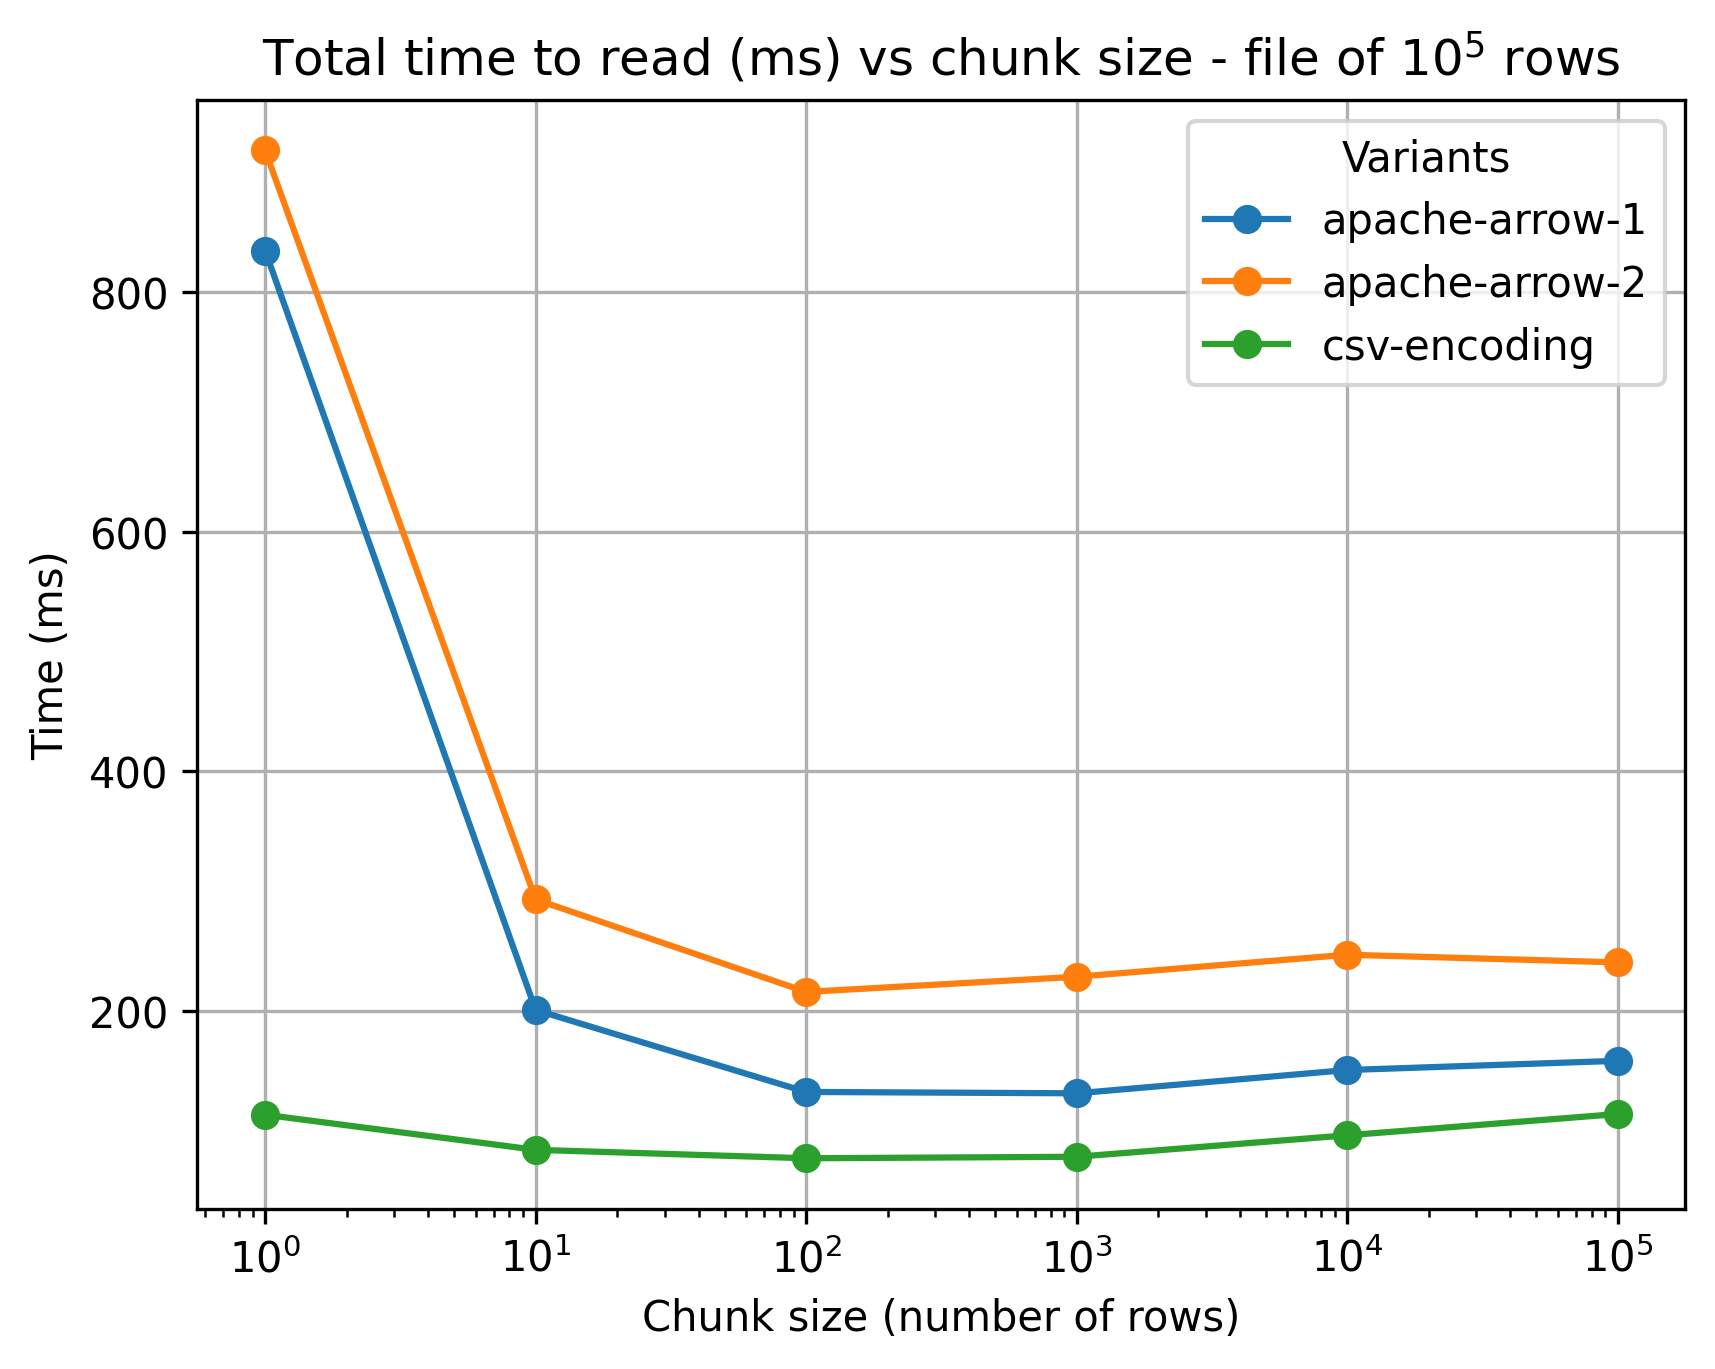
\includegraphics[scale = 0.7]{images/4-Experiments/read-input-10-5.png}
  \caption{Comparison of the variants for file of $10^5$ rows}
\end{figure}

\begin{figure}[H]
  \centering
  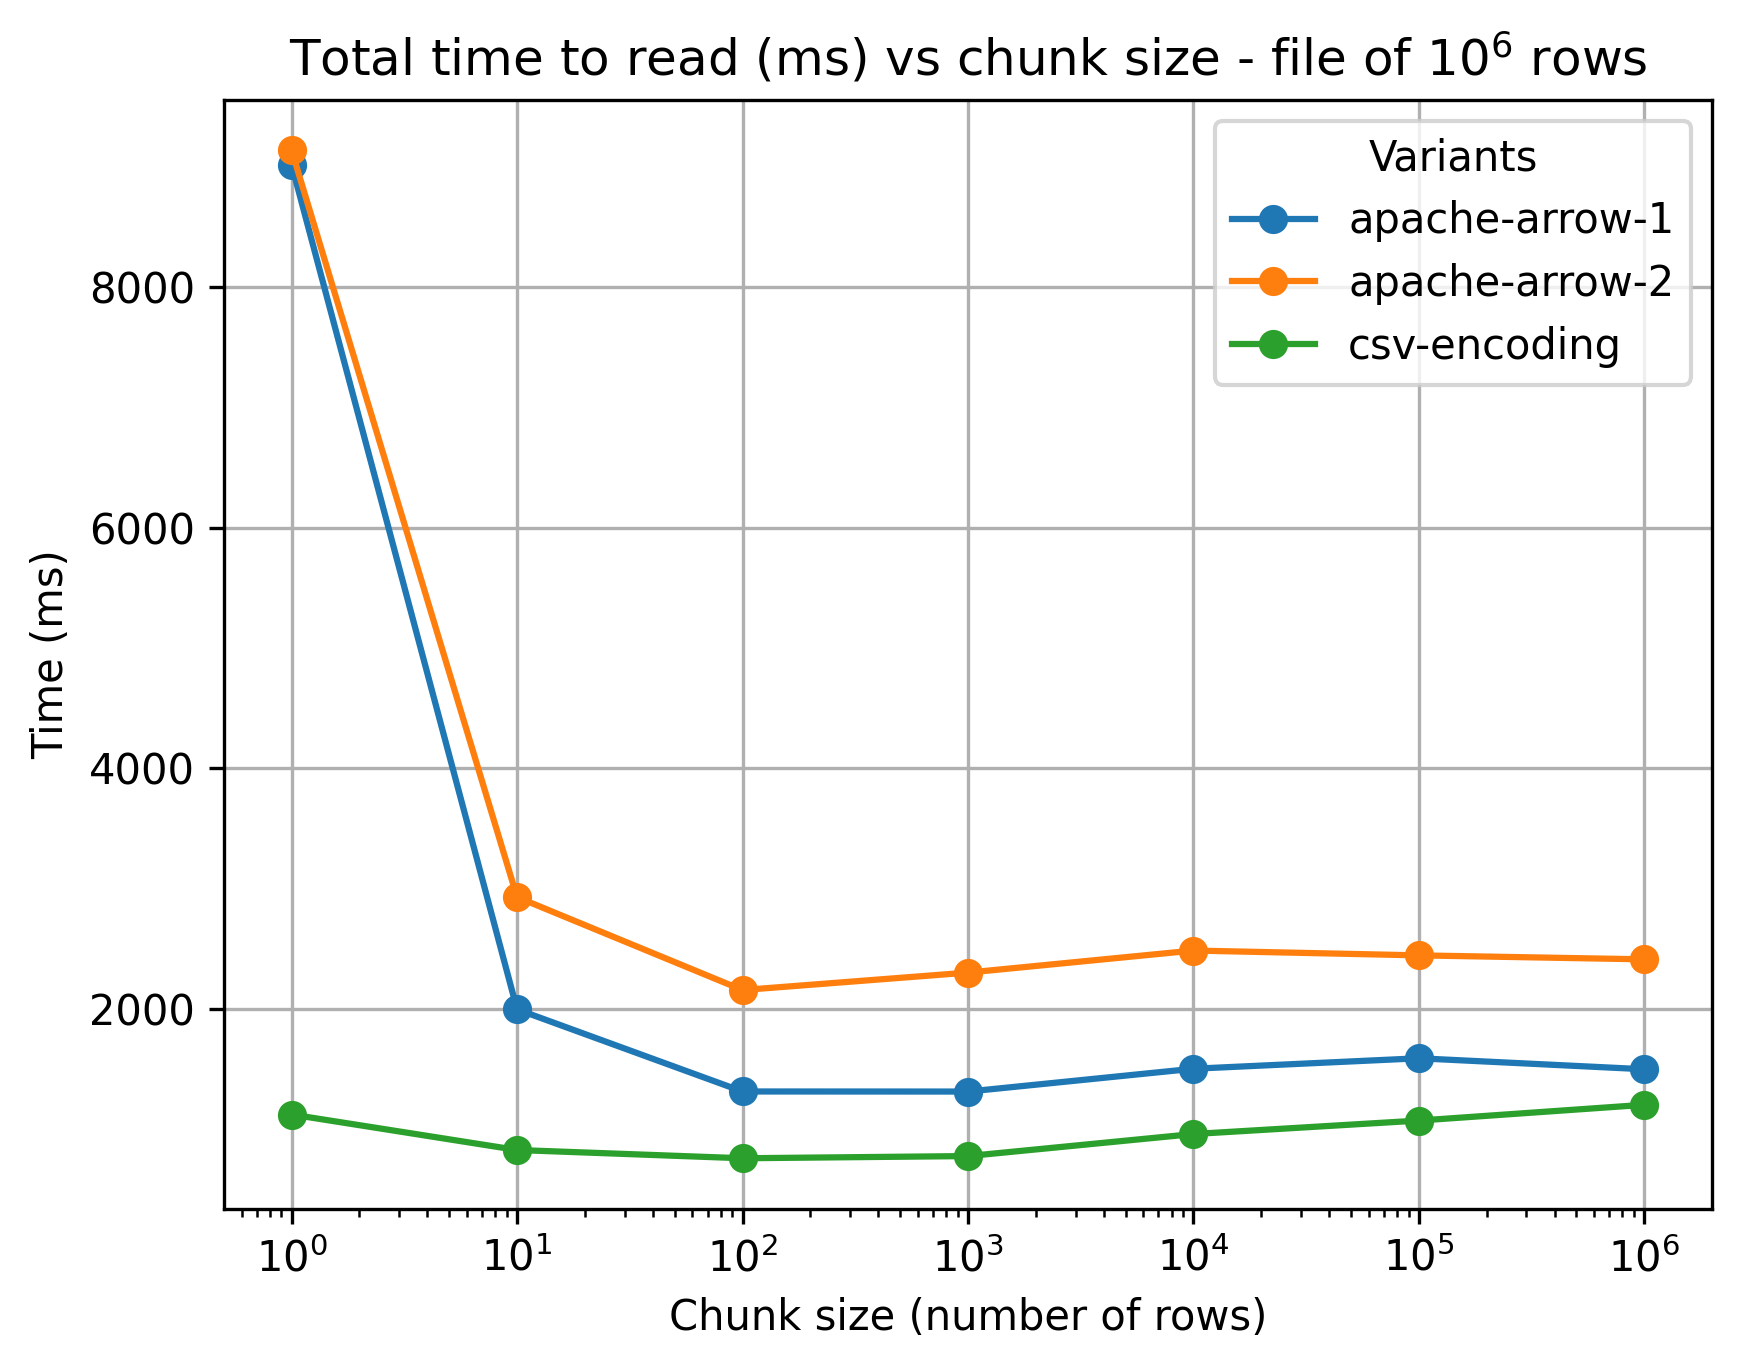
\includegraphics[scale = 0.7]{images/4-Experiments/read-input-10-6.png}
  \caption{Comparison of the variants for file of $10^6$ rows}
\end{figure}

Note that in all of the cases, the fastest approach is the one using the \texttt{csv/encoding} library. And, in addition, with chunk size of $10^2$ rows.

Once we decided to use the approach using the \texttt{csv/encoding} library, we performed an additional experiment in order to see if it was actually worthy to do the \emph{background} reading of the input with a worker goroutine. To see this:

\begin{itemize}
  \item Compare the variant with worker and chunk size of $10^2$ with the one without worker and therefore not reading by chunks.
  \item Comparison for different sizes of files: $10^4$, $10^5$ and $10^6$ number of rows (transactions).
  \item Each of the experiments is done 20 times to obtain stable measurements.
\end{itemize}

\begin{figure}[H]
  \centering
  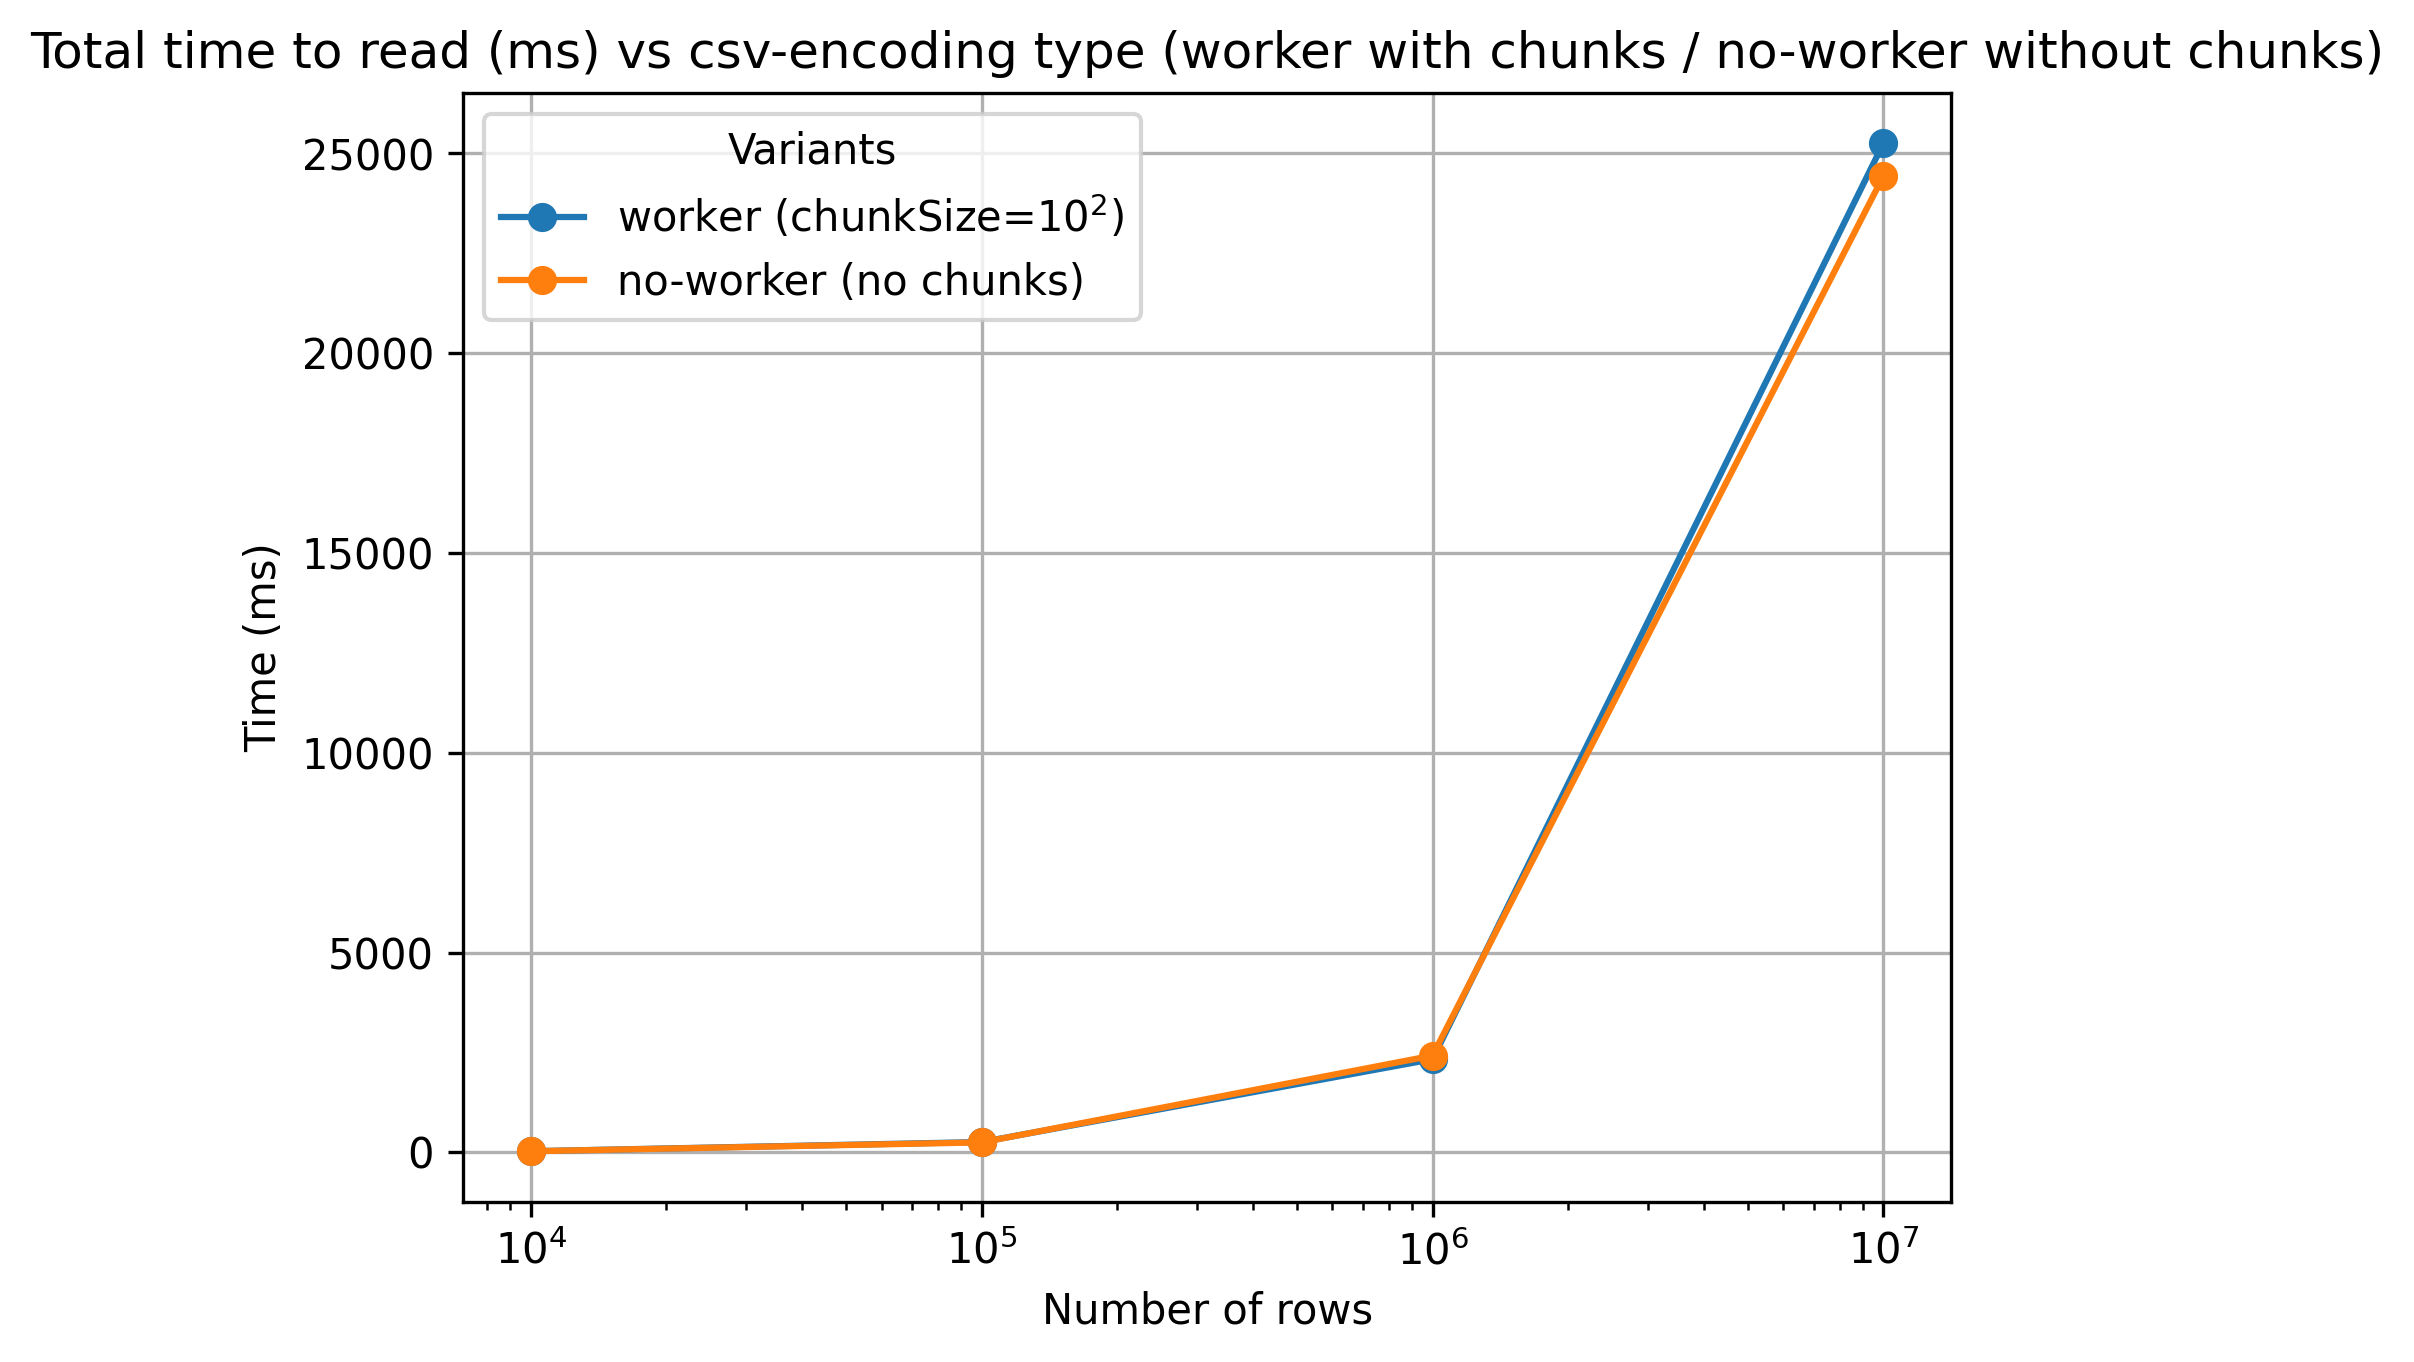
\includegraphics[scale = 0.7]{images/4-Experiments/read-input-csv-encoding-all.png}
  \caption{Comparison of \texttt{csv/encoding} variants up to $10^7$ rows}
\end{figure}

\begin{figure}[H]
  \centering
  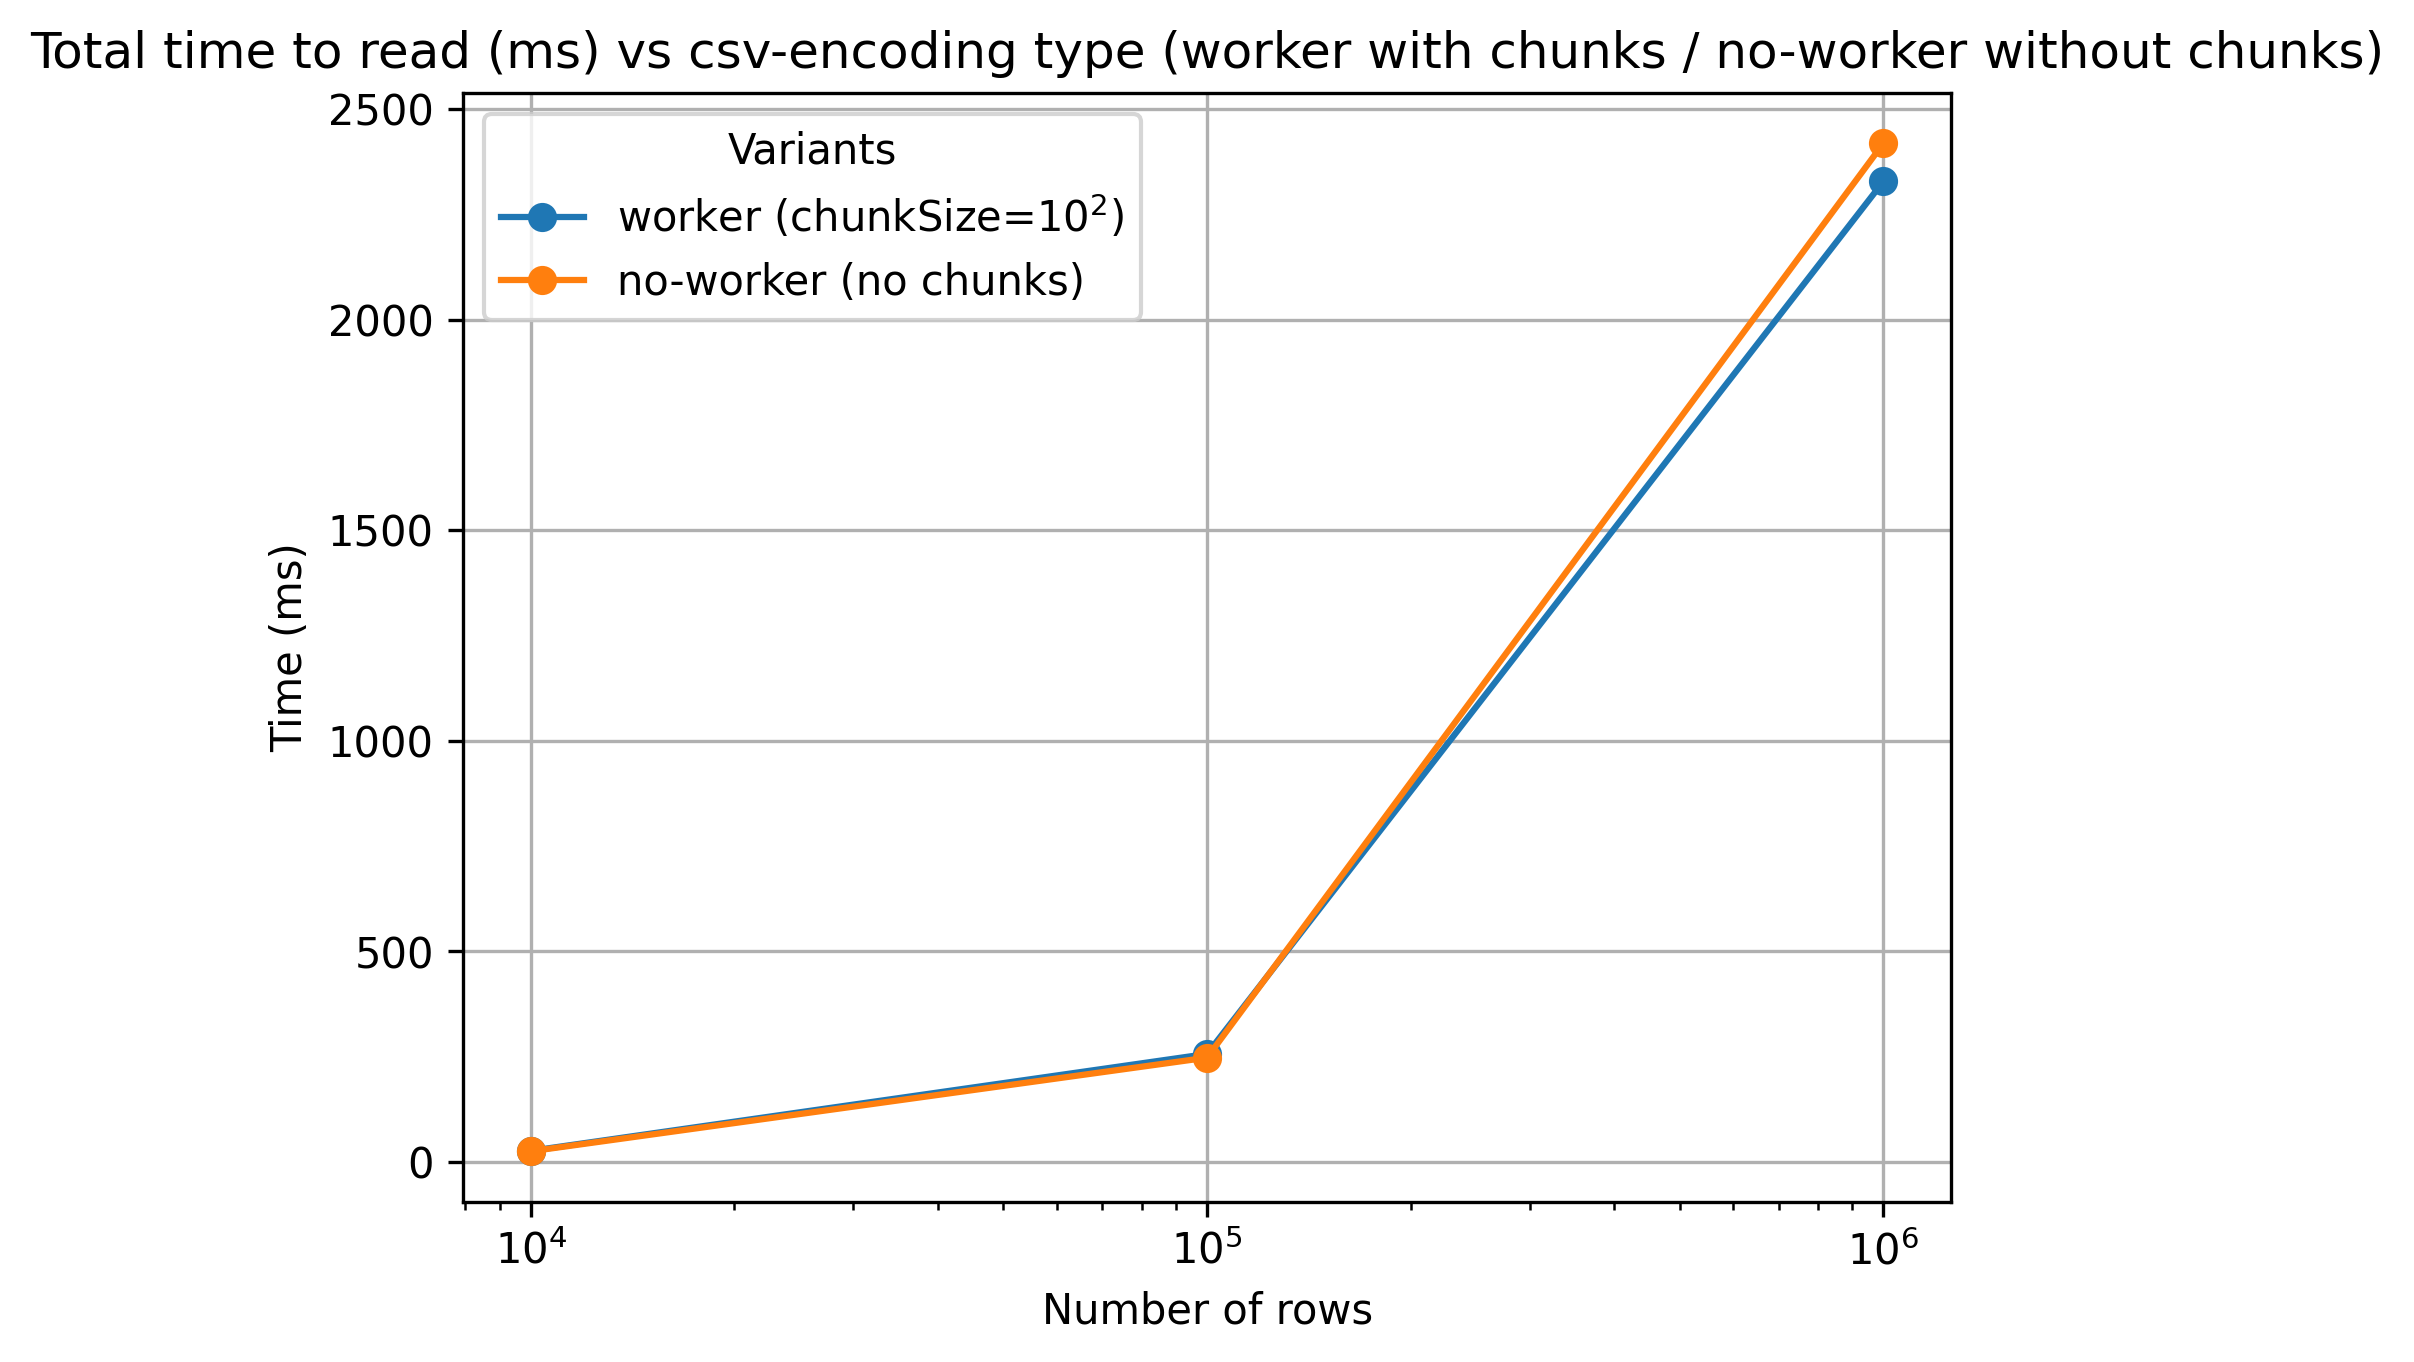
\includegraphics[scale = 0.7]{images/4-Experiments/read-input-csv-encoding.png}
  \caption{Comparison of \texttt{csv/encoding} variants up to $10^6$ rows}
\end{figure}

\begin{itemize}
  \item Differences insignificant
  \item Depend on the application
  \item Real-time simulation: worker version. To avoid possible bottleneck on the input reading. Instead the bottleneck be just the stopping to provide the input.
\end{itemize}

\textcolor{blue}{As it can be seen, the differences are insignificant, and the selection of each of the variants will depend on the application. For example, we suspect that the worker version can be beneficial in the real time simulation, so that we do not make the reading be the bottleneck of the simulation, by having a background process reading input transactions from the stream files while the main process providing the input to the pipeline can be stopped doing the real time simulation.}

\textcolor{red}{TODO: Comparativa run same experiment NRT with worker VS without worker for the input providing - a single experiment example to show that is better with worker!}

Some (other) references:

\begin{itemize}
  \item \href{https://www.confluent.io/es-es/learn/apache-flink/}{Apache Flink}: distributed processing engine for stateful computation of data streams.
\end{itemize}

\subsection{Experimental Approaches}

Note that, because of the way we did the transaction generator (coming from wisabi database client's behavior), the average number of transactions per day per card is $\sim1$, and therefore to be able to generate a transaction set with anomalous situations more close to reality, a reasonable time interval size for the generated transaction stream would be having $T$ around some weeks or month(s).

\begin{itemize}
\item{E1: Mean Response Time}

\begin{itemize}
  \item Q1: How much it takes for the system to emit the alerts from the moment the anomalous transaction was produced.
  \item R1: Real time simulation. Measuring the mean response time from the start of the transaction of the detected anomalous scenario until the alert is emitted by the system.
\end{itemize}

\item{E2: Continuous delivery of results in a high loaded scenario}

\begin{itemize}
  \item Q2: Behavior of the different system variations on a high loaded transaction stream scenario.
  \item R2: Not real time simulation. Direct transaction stream input supply. Comparison of the continuous delivery of results of the different systems variations (diefficiency metrics).
\end{itemize}
\end{itemize}

\subsubsection{E1: Mean Response Time}

\textbf{Real time-event stream simulation\\}
Since we do not have the material time to run each experiment for a interval time $T$ of some weeks or a month the idea is to do time scaling of the time event stream. We take the stream of a certain time interval size $T$ and map it into a smaller time interval
$T'$ where $T' << T$. Then, we do a real-time event simulation, providing the events of the input stream to the system at the times they actually occur (in reality possibly with a small certain delay!) using their timestamps.

\begin{itemize}
  \item \textbf{Shorter experimental time}: Reduced time to test the system behavior. Instead of $T$, only $T'$ time to test it. 
  \item \textbf{Stress testing - Graph database size - amount of filters' subgraphs}: We do not test the system under a real-case scenario considering its number of cards $c$, instead we are testing it under a higher load to what it would correspond, but having $c$ cards, and therefore $c$ filter's subgraph. The benefit is that we do not need to have such a big graph database.
\end{itemize}

The consequences for the experiments and metrics:

\begin{itemize}
  \item \textbf{Diefficiency metrics} (continuous delivery of results): If we give the input stream to the system respecting the temporal timestamps, note that no matter the system characteristics, that a result (an alert in our case), will not be possible to be produced until the event causing it arrives to the system. Therefore the emission of events is expected to be really similar in this case, for any system variation. Only in the case when the stream load is high enough we expect to see some differences?? \textcolor{orange}{$\rightarrow$ HABRÁ QUE IR VIÉNDOLO...}
  \item \textbf{Response time}: having in mind the previous considerations, we think in measuring the possible differences of behavior of the different system capabilities in terms of the mean response time. The mean response time (\texttt{mrt}) would be the average time that the system spends since it receives the transactions involved in an alert until the time it emits the alert.
\end{itemize}

\textcolor{red}{Problems derived to pay attention to}:
\begin{itemize}
  \item Shrinking the timestamps to a smaller time interval, produces the emergence of not real fraud patterns that before did not exist due to their real and "correct" larger time distance. Example:
  \begin{itemize}
  \item Consider the original size of the time interval of the input stream $T=120h$ (5 days) and $T'=24h$.
  \item Consider two consecutive regular transactions of a certain client performed in two different ATMs \texttt{ATM-x} and \texttt{ATM-y} with \texttt{t\_min}$=8$h (minimum time difference to traverse the distance from \texttt{ATM-x} to \texttt{ATM-y}) and \texttt{t\_diff}$=24$h (time difference between the first and the second transaction). 
  \item \textcolor{red}{$\rightarrow$ Note that with the scaling the time difference \texttt{t\_diff} would be of 5 times less, that is, $\texttt{t\_diff}=4.8h$. Therefore this will make $\texttt{t\_diff'}=4.8h < \texttt{t\_min}=8h$}.
  \end{itemize}
  \item $\rightarrow$ (*) Solution A: \textbf{introduce the scaling factor as a input parameter} and consider it also for the fraud checking so to properly \textbf{scale the $\texttt{t\_min}$ variable} ($\texttt{t\_min}=8h \rightarrow \texttt{t\_min'}=\frac{8}{5}h=1.6h$) and therefore: 
  \begin{itemize}
    \item Before scaling: $\texttt{t\_diff}=24h > \texttt{t\_min}=8h$.
    \item After scaling (scale factor $=\frac{1}{5}$): $\texttt{t\_diff}=24*\frac{1}{5}=4.8h > \texttt{t\_min}=8*\frac{1}{5}=1.6h$.
  \end{itemize}
  \item $\rightarrow$ Solution B: conserve the original timestamps, and consider the mapped-reduced timestamps for simulating the arrival times of the transactions into the system while taking the original timestamps for the checking of the frauds.
\end{itemize}

\begin{tcolorbox}[colframe=red!75]
\textcolor{red}{\textbf{IMPORTANT: WHAT DO WE WANT TO TEST?\\}}
Definition of the objectives of the experiments:
\begin{itemize}
    \item See and compare the behavior of the system(s) with different streams (different number of cards, greater or smaller size of the bank - and therefore its database). \\
    \begin{itemize}
        \item Alert/result response time comparison. \textbf{Continuous delivery of results (diefficiency metrics) does not make sense!}. With the objective to see that we can see lower response time in the case of the dp versions.
    \end{itemize}
\end{itemize}
\end{tcolorbox}

\paragraph{Problems derived:\\}
\begin{itemize}
    \item \textbf{Continuous delivery of results comparison does not make sense.} $\rightarrow$ In a real time simulation, for any system, results can only be emitted whenever the corresponding anomalous transaction $a_i$ reaches the system. That happens at the same time $t_i$ for both approaches when the input stream is simulated at real time, meaning that the result corresponding to the anomalous transaction $a_i$ can not be emitted in any case before time $t_i$. Therefore, the difference in time delivery of this result between the different approaches is not expected to be high unless we make the systems to be loaded enough. \textbf{Therefore, for small sized banks this does not really make sense...}
    \item \textbf{Losing of alerts}: Due to scaling we are losing alerts since we have seconds precision. We will have to scale to the millisecond or nanosecond the timestamps to possibly do not loose those alerts, due to time scaling precision.
    \item \textbf{Although scaling, the load we are simulating is higher than real... - like for the not real time approach}
\end{itemize}

\subsubsection{E2: Continuous delivery of results in a high loaded scenario}

Do not consider the real-time simulation, by omitting the transaction timestamps in the sense that we do not consider them to simulate a real case scenario where each transaction arrives to the system at the time indicated by its timestamp. 
Instead all the stream comes (ordered by timestamp) but directly (almost) at the same time to the system. With this approach:
\begin{itemize}
  \item \textbf{No real case simulation}
  \item \textbf{Measure the load the system can take}: for the different system variations given a same stream.
  \item \textbf{Diefficiency metrics}: since time arrival of the transactions to the system is now ignored, and all the transactions come one after the other, a result to be produced do not need to wait for the real timestamp of the transaction. Therefore, we could see the differences in continuously delivering results of the different systems under the same input stream load (more clear than before).
\end{itemize}

\begin{tcolorbox}[colframe=red!75]
\textcolor{red}{\textbf{IMPORTANT: WHAT DO WE WANT TO TEST?\\}}
Definition of the objectives of the experiments:
\begin{itemize}
    \item See and compare the behavior of the system(s) with different streams (different number of cards, greater or smaller size of the bank - and therefore its database). \\
    \textcolor{teal}{Objective: see that the dp approach is better to handle bigger stream sizes.}
    \begin{itemize}
        \item Continuous delivery of results comparison (diefficiency metrics).
        \item Total execution time needed to process the full stream.
        \item Maximum endurance capacity of the system(s) -- until which size of stream can the system work without crashing (\textit{Hasta donde podemos llegar a aguantar con nuestro sistema. Capacidad de carga máxima.})
    \end{itemize}
\end{itemize}
\end{tcolorbox}

\paragraph{Problems derived:\\}
\begin{itemize}
    \item \textbf{The load we are simulating is way higher than real (of course higher than for the real time approach)}
    \item \textbf{The reading of the input can be our bottleneck}: Try to find the fastest way to deal with it (described in \ref{input-reading}).    
\end{itemize}

\textbf{What we do then?}
$\rightarrow$ Try both kinds of experiments. 
For the first:
\begin{itemize}
    \item Document what I have and explain what I have seen so far.
    \item Continue running some more to see if I can see more differences. With more transactions and stream load.
    \item Try to scale to the millisecond/nanosecond timestamp precision. See if I can avoid losing alerts.
\end{itemize}
For the second:
--- START THEM, following the variations in the notebook (already explained)---

\subsection{Experiments description}

Initially, we take as reference some small Spanish banks, such as "Caja Rural de Aragón" with:
\begin{itemize}
  \item $|ATM| \sim 200$
  \item $|Card| \sim 14000$
\end{itemize}

other small banks have $|ATM| \sim 200$ and around up to $|Card| \sim 10^{5}$.
\textit{Note that, for simplicity, we are assuming the number of bank branches as the number of ATMs and the number of clients as the number of cards.}
\textcolor{red}{TODO: PONER enlace a web de donde obtengo estos datos!}


Regarding the size of the transaction stream, looking at some related works such as:
\textcolor{red}{TODO: PONER ESTAS REFERENCIAS}
work with a transaction stream of a size around $\sim 10^{5},10^{6}$.

For the transaction stream size we need to consider that our transaction generator takes as base the behavior of the clients of the 
Wisabi Bank Database, where each client typically produces at most $\sim 1$ transaction per day. (\textcolor{red}{TO CHECK to give the exact number}).

In relation with the fraud ratio, some works like \textcolor{red}{TODO: PONER ESTAS REFERENCIAS} were reviewed...

\subsubsection{Initial experiments}

\textit{Small} initial graph database (gdb) size:
\begin{itemize}
  \item $|ATM| = 50$
  \item $|Card| = 2000$
\end{itemize}

Transaction stream:
\begin{itemize}
  \item $\texttt{NUM\_DAYS} = 30$
  \item $\texttt{anomalous\_ratio} = 0.02\ (2\%)$ 
\end{itemize}

This setup gives us a transaction stream of 
\begin{itemize}
  \item $\texttt{total\_tx} = 39959$
  \item $\texttt{regular\_tx} = 39508$
  \item $\texttt{anomalous\_tx} = 451$ -- note that this is actually a $1\%$.
\end{itemize}

\begin{table}[H]
\centering
\begin{tabular}{|c|c|c|c|c|c|}
  \hline
  Execution & Scaled   & Num. cards/filter& Num. cores & Num. alerts & Time(s) \\ \hline
  NRT & No & Baseline (all) & 1 & 462 & 44.88 \\ \hline
  RT  & 1h & Baseline (all) & 1 & 447 & 3601.65\\ \hline
  RT  & 1h & 500 (4 filters) & 4 & 447 & 3603.25\\ \hline
  RT  & 1h & 200 (10 filters) & 10 & 447 & 3602.71\\ \hline
  RT  & 6h & Baseline (all) & 1 & 459 & 21606.11 \\ \hline
  RT  & 6h & 500 (4 filters) & 4 & 459 & 21611.75 \\ \hline
  RT  & 12h & Baseline (all) & 1 & 461 & 43211.95 \\ \hline
\end{tabular}
\caption{Different experimental setups results}
\label{table:small-results}
\end{table}

Some nomenclature:
\begin{itemize}
  \item NRT: Not Real Time execution
  \item RT: Real Time execution
\end{itemize}

Some results:

\paragraph{1h scaling\\}


\begin{figure}[H]
  \centering
  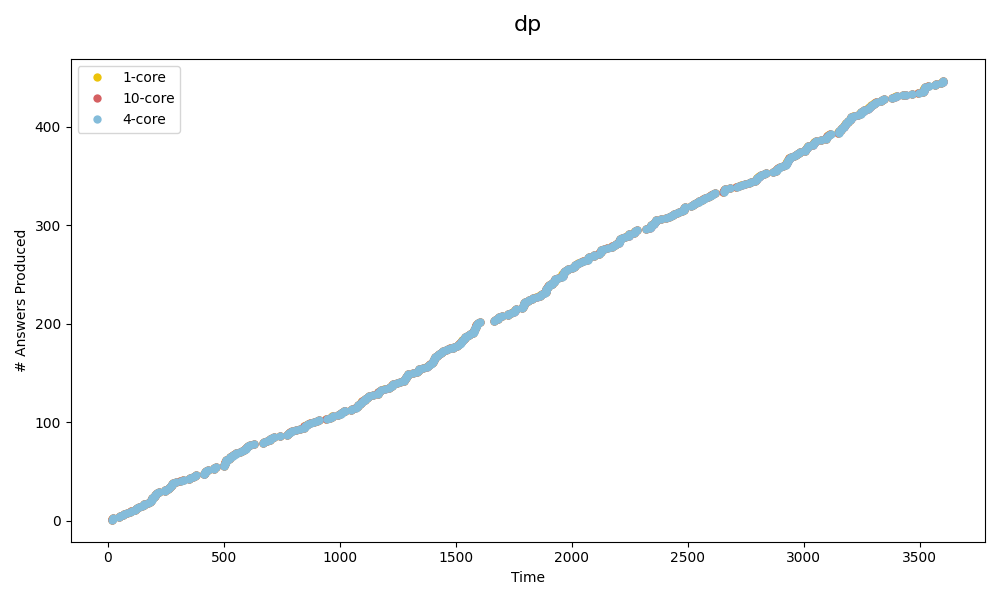
\includegraphics[scale = 0.5]{images/4-Experiments/traces-1h.png}
  \caption{Trace 1h}
\end{figure}

Only for the first 10 results (alerts):
\begin{figure}[H]
  \centering
  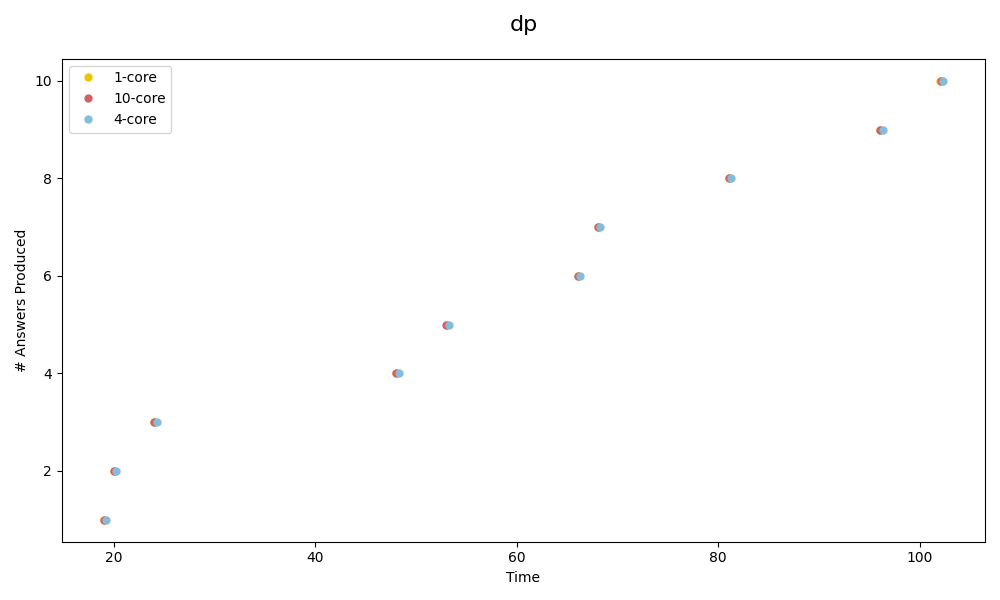
\includegraphics[scale = 0.5]{images/4-Experiments/traces-1h-10.png}
  \caption{Trace 1h - first 10 alerts}
\end{figure}

\paragraph{6h scaling\\}

We do not see any difference in the behavior between the baseline with 1 filter and 1 core approach (\texttt{RT-6h-1c-1f}) and the approach with 4 filters and 4 cores (\texttt{RT-6h-4c-4f}). 

\textbf{WHY?} $\rightarrow$ a possible reason is that results can only be emitted whenever the corresponding anomalous transaction $a_i$ reaches the system. That happens at the same time $t_i$ for both approaches when the input stream is simulated at real time, meaning that the result corresponding to the anomalous transaction $a_i$ can not be emitted in any case before time $t_i$. Therefore, the difference in time delivery of this result between the different approaches is not expected to be high unless we make the systems to be loaded enough.


\subsection{E2: Continuous delivery of results in a high loaded scenario}

\begin{itemize}
  \item Q2: Behavior of the different system variations on a high loaded transaction stream scenario.
  \item R2: Not real time simulation. Direct transaction stream input supply. Comparison of the continuous delivery of results of the different systems variations (diefficiency metrics).
\end{itemize}

$\rightarrow$ We set the worker stream reading by chunks, with chunk size of $10^2$.\\

The setups of the experiments that we are going to do are:
\begin{itemize}
  \item Fix different bank sizes (small, $+\frac{1}{4}$, $+\frac{2}{4}$, $+\frac{3}{4}$, the biggest possible size).
  \begin{itemize}
    \item For each, generate different stream sizes.
    \begin{itemize}
      \item Compare different system variations in the number of cores and number of filters.
    \end{itemize}
  \end{itemize}
\end{itemize}

\subsubsection{Bank size: Initial - Small}

\begin{itemize}
  \item $|ATM| = 50$
  \item $|Card| = 2000$
\end{itemize}

\paragraph{Transaction stream - small\\}

\begin{itemize}
  \item $\texttt{NUM\_DAYS} = 30$
  \item $\texttt{anomalous\_ratio} = 0.02\ (2\%)$ 
\end{itemize}

This setup gives us a transaction stream of 
\begin{itemize}
  \item $\texttt{total\_tx} = 39959$
  \item $\texttt{regular\_tx} = 39508$
  \item $\texttt{anomalous\_tx} = 451$ -- note that this is actually a $1\%$.
\end{itemize}

For different core variations, we are going to try different combinations of the system in terms
of the number of the maximum number of cards per filter, that consequently will produce an inverse variation in the number of filters of the system.

\begin{table}[H]
  \renewcommand{\arraystretch}{1.5} % control row height
  \centering
  \begin{tabular}{|c|c|}
  \hline
  \# cards per filter & \# filters \\ \hline
  $|Card|\ / \ {2^0} $  &   1     \\ \hline
  $|Card|\ / \ {2^1} $ &   2     \\ \hline
  $|Card|\ / \ {2^2} $ &   4     \\ \hline
  $|Card|\ / \ {2^3} $ &   8     \\ \hline
  $|Card|\ / \ {2^4} $ &   16    \\ \hline
  $|Card|\ / \ {2^5} $ &   32    \\ \hline
  \end{tabular}
\end{table}

\begin{itemize}
  \item \# of times / runs each job $=10$.
  \item Maximum RAM limited to 16GB.
\end{itemize}

\paragraph{1-core\\}

Results for executions with 1-core:

\begin{figure}[H]
  \centering
  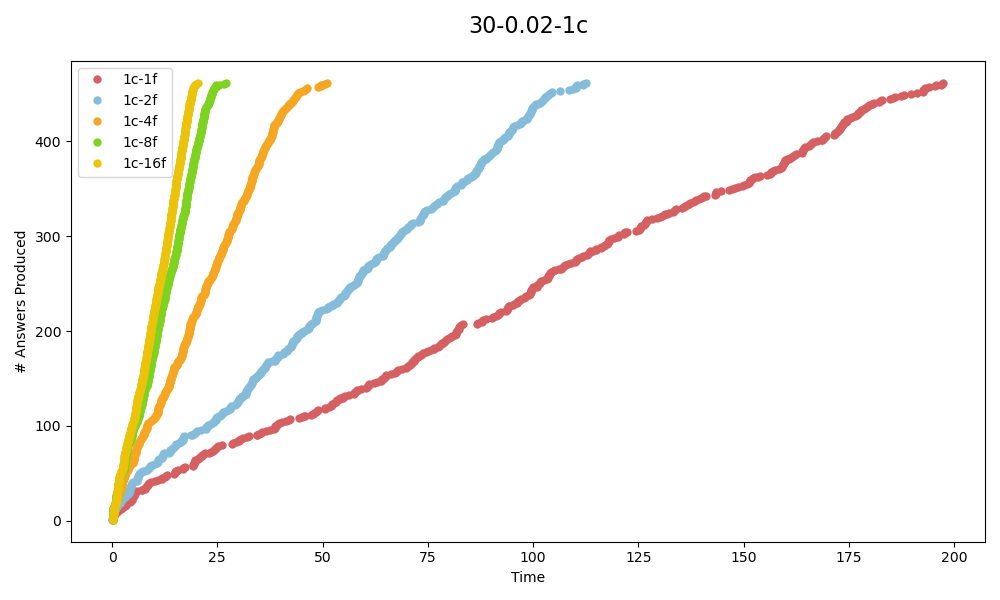
\includegraphics[scale = 0.5]{images/4-Experiments/E2/30-0.02-1c/traces.png}
  \caption{Alerts trace in time (s) - 1 core}
\end{figure}

\begin{figure}[H]
  \centering
  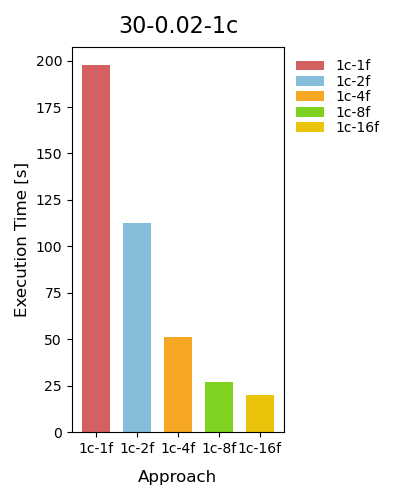
\includegraphics[scale = 0.5]{images/4-Experiments/E2/30-0.02-1c/execTime.png}
  \caption{Execution time (s) - 1 core}
\end{figure}

\begin{figure}[H]
  \centering
  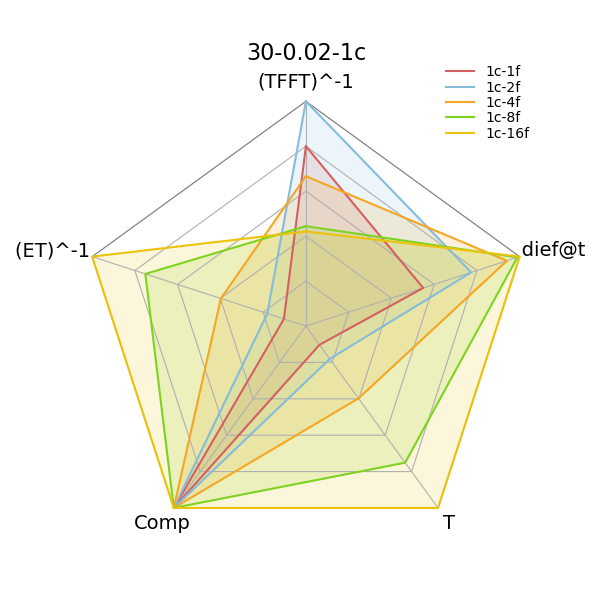
\includegraphics[scale = 0.5]{images/4-Experiments/E2/30-0.02-1c/radar-dieft.png}
  \caption{\texttt{dieft} radar - 1 core}
\end{figure}

\begin{figure}[H]
  \centering
  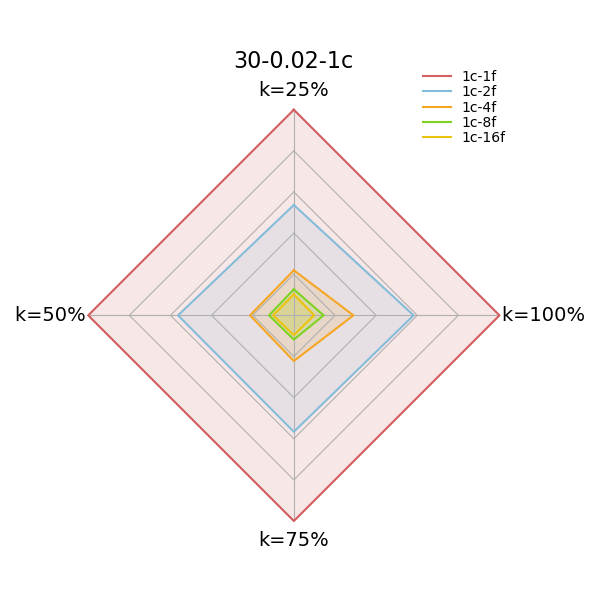
\includegraphics[scale = 0.5]{images/4-Experiments/E2/30-0.02-1c/radar-diefk.png}
  \caption{\texttt{diefk} radar - 1 core}
\end{figure}

\textcolor{red}{TODO: Put table for not graphical results gathered in the dieffpy-out.txt file...}

\paragraph{4-cores\\}

Results for executions with 4-core:

\begin{figure}[H]
  \centering
  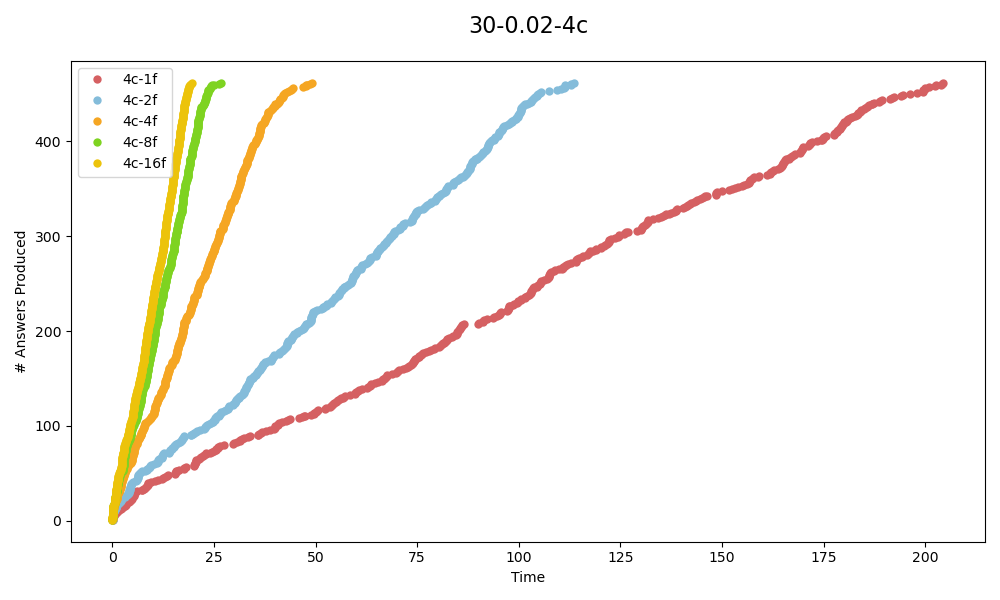
\includegraphics[scale = 0.5]{images/4-Experiments/E2/30-0.02-4c/traces.png}
  \caption{Alerts trace in time (s) - 4 core}
\end{figure}

\paragraph{8-cores\\}

Results for executions with 8-core:

\begin{figure}[H]
  \centering
  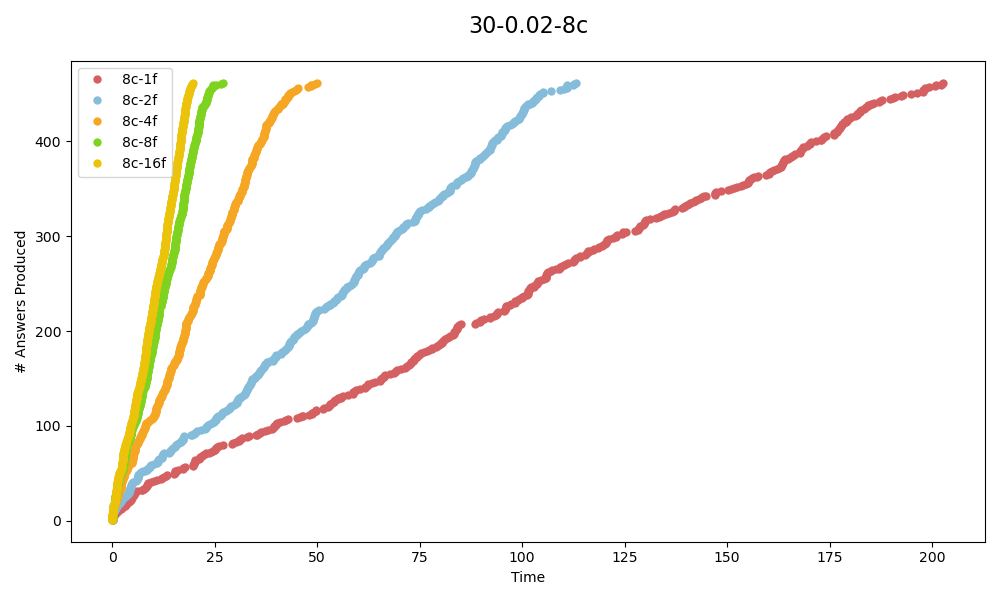
\includegraphics[scale = 0.5]{images/4-Experiments/E2/30-0.02-8c/traces.png}
  \caption{Alerts trace in time (s) - 8 core}
\end{figure}

\paragraph{16-cores\\}

Results for executions with 16-core:

\begin{figure}[H]
  \centering
  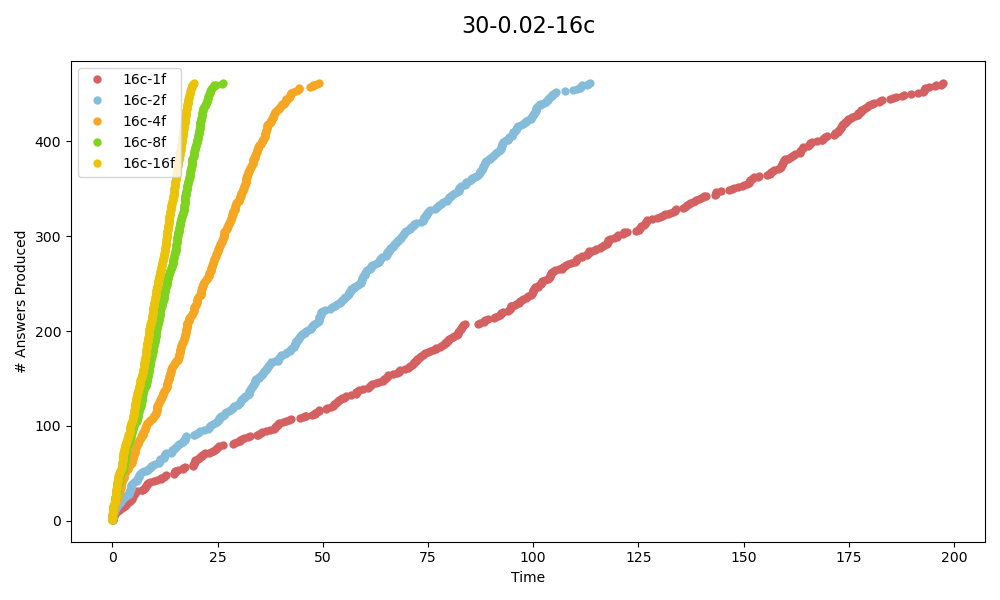
\includegraphics[scale = 0.5]{images/4-Experiments/E2/30-0.02-16c/traces.png}
  \caption{Alerts trace in time (s) - 16 core}
\end{figure}

\textcolor{red}{NOTE: Almost no difference when variating the number of cores!!!!}

\begin{figure}[H]
  \centering
  \begin{subfigure}[b]{0.45\textwidth}
    \centering
    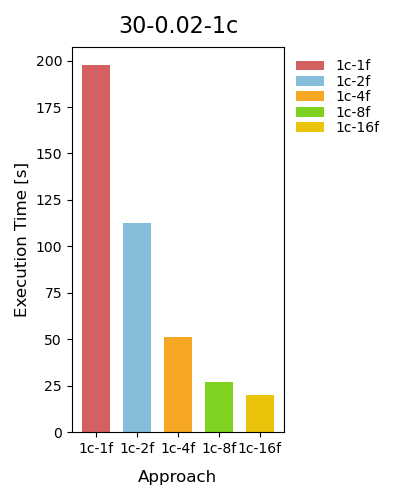
\includegraphics[scale=0.6]{images/4-Experiments/E2/30-0.02-1c/execTime.png}
    \caption{Execution time (s) - 1 core}
  \end{subfigure}
  \hfill
  \begin{subfigure}[b]{0.45\textwidth}
    \centering
    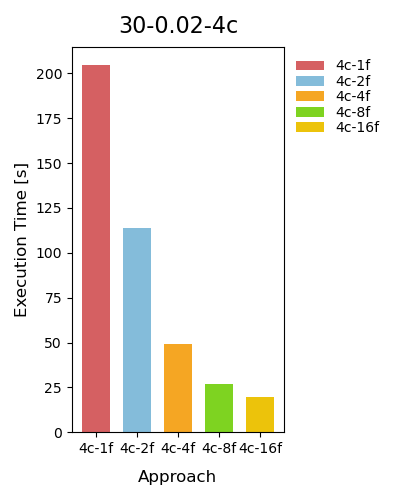
\includegraphics[scale=0.6]{images/4-Experiments/E2/30-0.02-4c/execTime.png}
    \caption{Execution time (s) - 4 core}
  \end{subfigure}
  \\
  \begin{subfigure}[b]{0.45\textwidth}
    \centering
    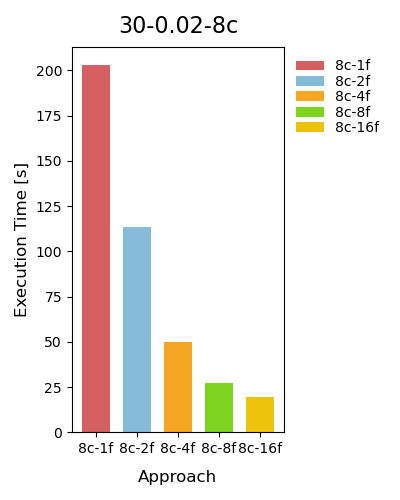
\includegraphics[scale=0.6]{images/4-Experiments/E2/30-0.02-8c/execTime.png}
    \caption{Execution time (s) - 8 core}
  \end{subfigure}
  \hfill
  \begin{subfigure}[b]{0.45\textwidth}
    \centering
    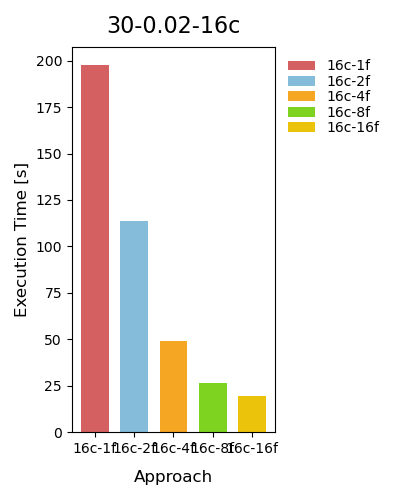
\includegraphics[scale=0.6]{images/4-Experiments/E2/30-0.02-16c/execTime.png}
    \caption{Execution time (s) - 16 core}
  \end{subfigure}
  \caption{Execution times for different core configurations.}
  \label{fig:execution-times}
\end{figure}

\paragraph{Transaction stream - medium\\}

\paragraph{Transaction stream - big\\}

\subsubsection{Bank size: $+\frac{1}{4}$ of Initial}

\subsection{How to run the experiments}

\begin{itemize}
    \item Run \texttt{\$> launchAll-\{1,2,4,...\}c.sh <descriptions> <execTimes>} where we select the script to run based on the number of cores (1,2,4...) and maximum RAM with which to run the set of experiments. Indicate the directory of the description files of the experiments to run with \texttt{<descriptions>}, and the number of times to run each experiment with the \texttt{<execTimes>} parameter.
    Each description file of an experiment has to be in a csv format indicating \texttt{txFile,test,approach,maxFilterSize} where:
    \begin{itemize}
        \item \texttt{txFile}: indicates the name of the input stream file.
        \item \texttt{test}: label indicating the name of the test we perform (stream input and cores)
        \item \texttt{approach}: label indicating the name of the approach we perform (cores and filters)
        \item \texttt{maxFilterSize}: to set the maximum number of cards per filter. To set up the maximum number of filters for the tested system.
    \end{itemize}
    An example of a csv experiment description file is shown in \ref{csv-exp-description}.
    \begin{center}
    \lstset{style=cypherStyle}
    \begin{lstlisting}[caption={30-0.02-1c-4f}, label={csv-exp-description}]
        txFile,test,approach,maxFilterSize
        ../input/small/30-0.02.csv,30-0.02-1c,1c-4f,500
    \end{lstlisting}
    \end{center}
    \item Run \texttt{\$> summary-results.sh <directory> <TEST>}: to obtain the averaged results of the experiments run stored in the indicated output \texttt{<directory>} (the predefined output directory is the called \texttt{output} directory) and then \texttt{<TEST>} where we need to indicate the name of the performed test (like in the experiments description files).
\end{itemize}
